\documentclass{beamer}
\usepackage{caption}
\usepackage{subcaption}
\usepackage{hyperref}
\usepackage{gensymb}
\usetheme{Madrid}
% \usetheme{Singapore}
\title{}
\author{Nithin}
\institute{}
\date{\today}
\begin{document}
\section{Nature of Light}
	\subsection{Propagation of Light}
\begin{frame}
	
 \frametitle{Ray Model of Light}
 3 ways light can travel from a source to another location
 	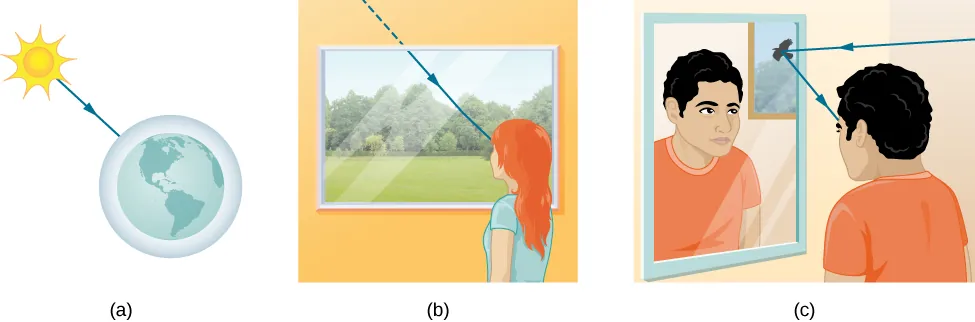
\includegraphics[width=10cm,height=3cm]{1.png}
 \begin{enumerate}
 	\item[a] directly from source through vaccum . Sun to Earth
 	\item[b] light can travel through various media like Air, glass, water to the observer 
 	\item[c] light can also arrive after being reflected such as mirrors
 \end{enumerate}

\end{frame}
\begin{frame}
\begin{block}{Ray of Light}
	We model path of light as a straight line called \alert{ray}
\end{block}
\begin{itemize}
	\item Light behaves both as a particle and a wave
	\item When light interacts with an object several times larger than its wavelength($\approx 10^{-6}$), it travels in a straight line and acts like a ray.
	\item Light may change direction when it 
	\begin{itemize}
		\item reflection : encounters objects (such as a mirror) 
		\item refraction: passing from one material to another (such as in passing from air to glass) 
	\end{itemize}	
\end{itemize}
\end{frame}
\subsection{Reflections}
\begin{frame}
	\begin{block}{Law of Reflection}
		the law states that agle of reflection is equal to angle of incidence
		\begin{displaymath}
			\theta_{r} = \theta_{i}
		\end{displaymath}
	\end{block}
	\begin{center}
		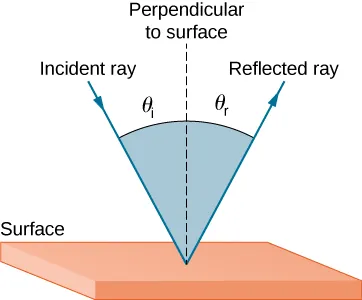
\includegraphics[width=5cm, height=5cm]{2.png}
	\end{center}
\end{frame}

\begin{frame}
	\begin{center}
		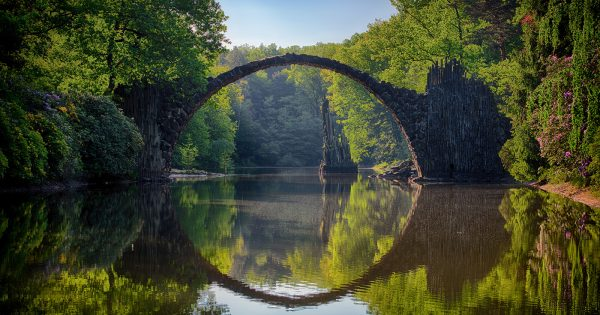
\includegraphics[scale=0.7]{3.jpg}
	\end{center}
\end{frame}

\begin{frame}
	\frametitle{Specular Reflection}
		\begin{center}
			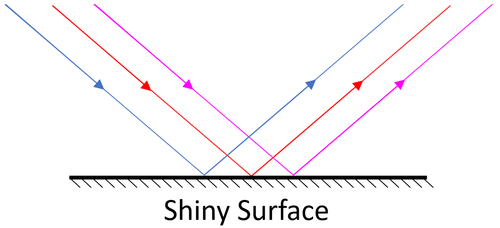
\includegraphics[scale=0.8]{6.png}
		\end{center}
\end{frame}
\begin{frame}
	\frametitle{Diffused Reflection}
		\begin{center}
			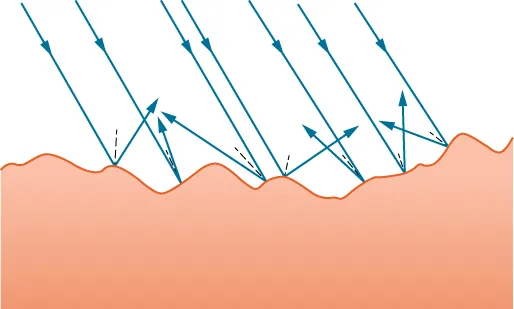
\includegraphics[scale=0.5]{5.png}
		\end{center}
\end{frame}

\begin{frame}
	\begin{center}
		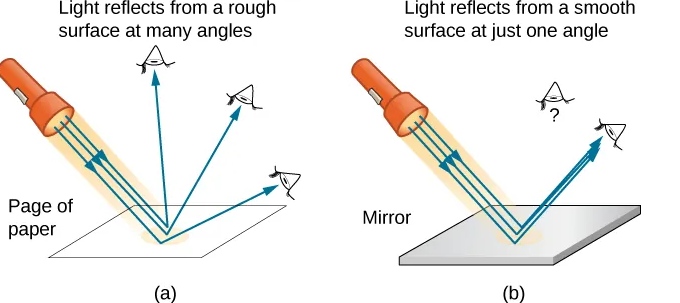
\includegraphics[scale=0.5]{8.png}
	\end{center}
\end{frame}
\begin{frame}
	\begin{center}
		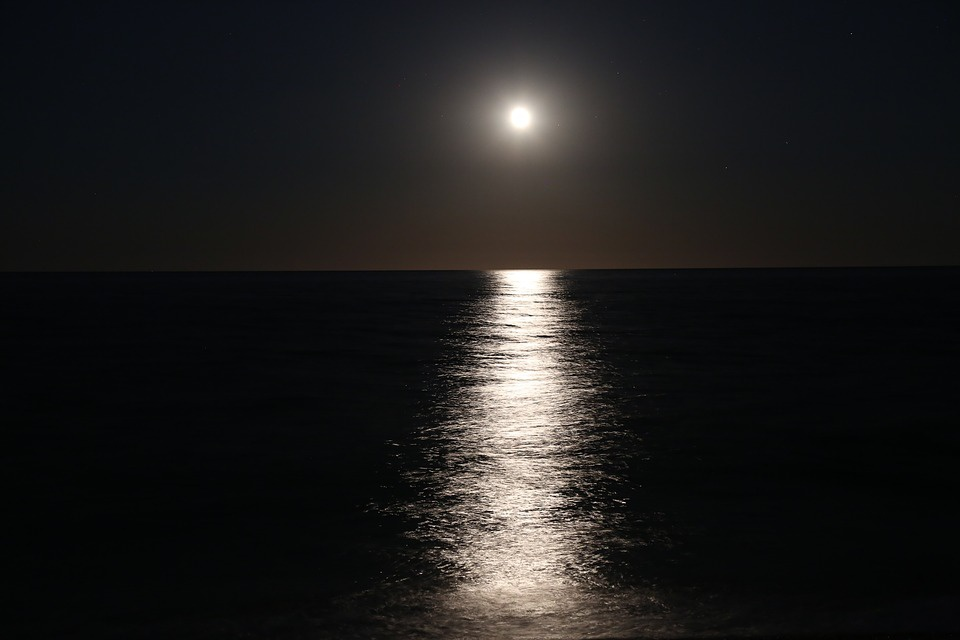
\includegraphics[scale=0.32]{9.jpeg}
	\end{center}
\end{frame}
\begin{frame}

	\begin{center}
		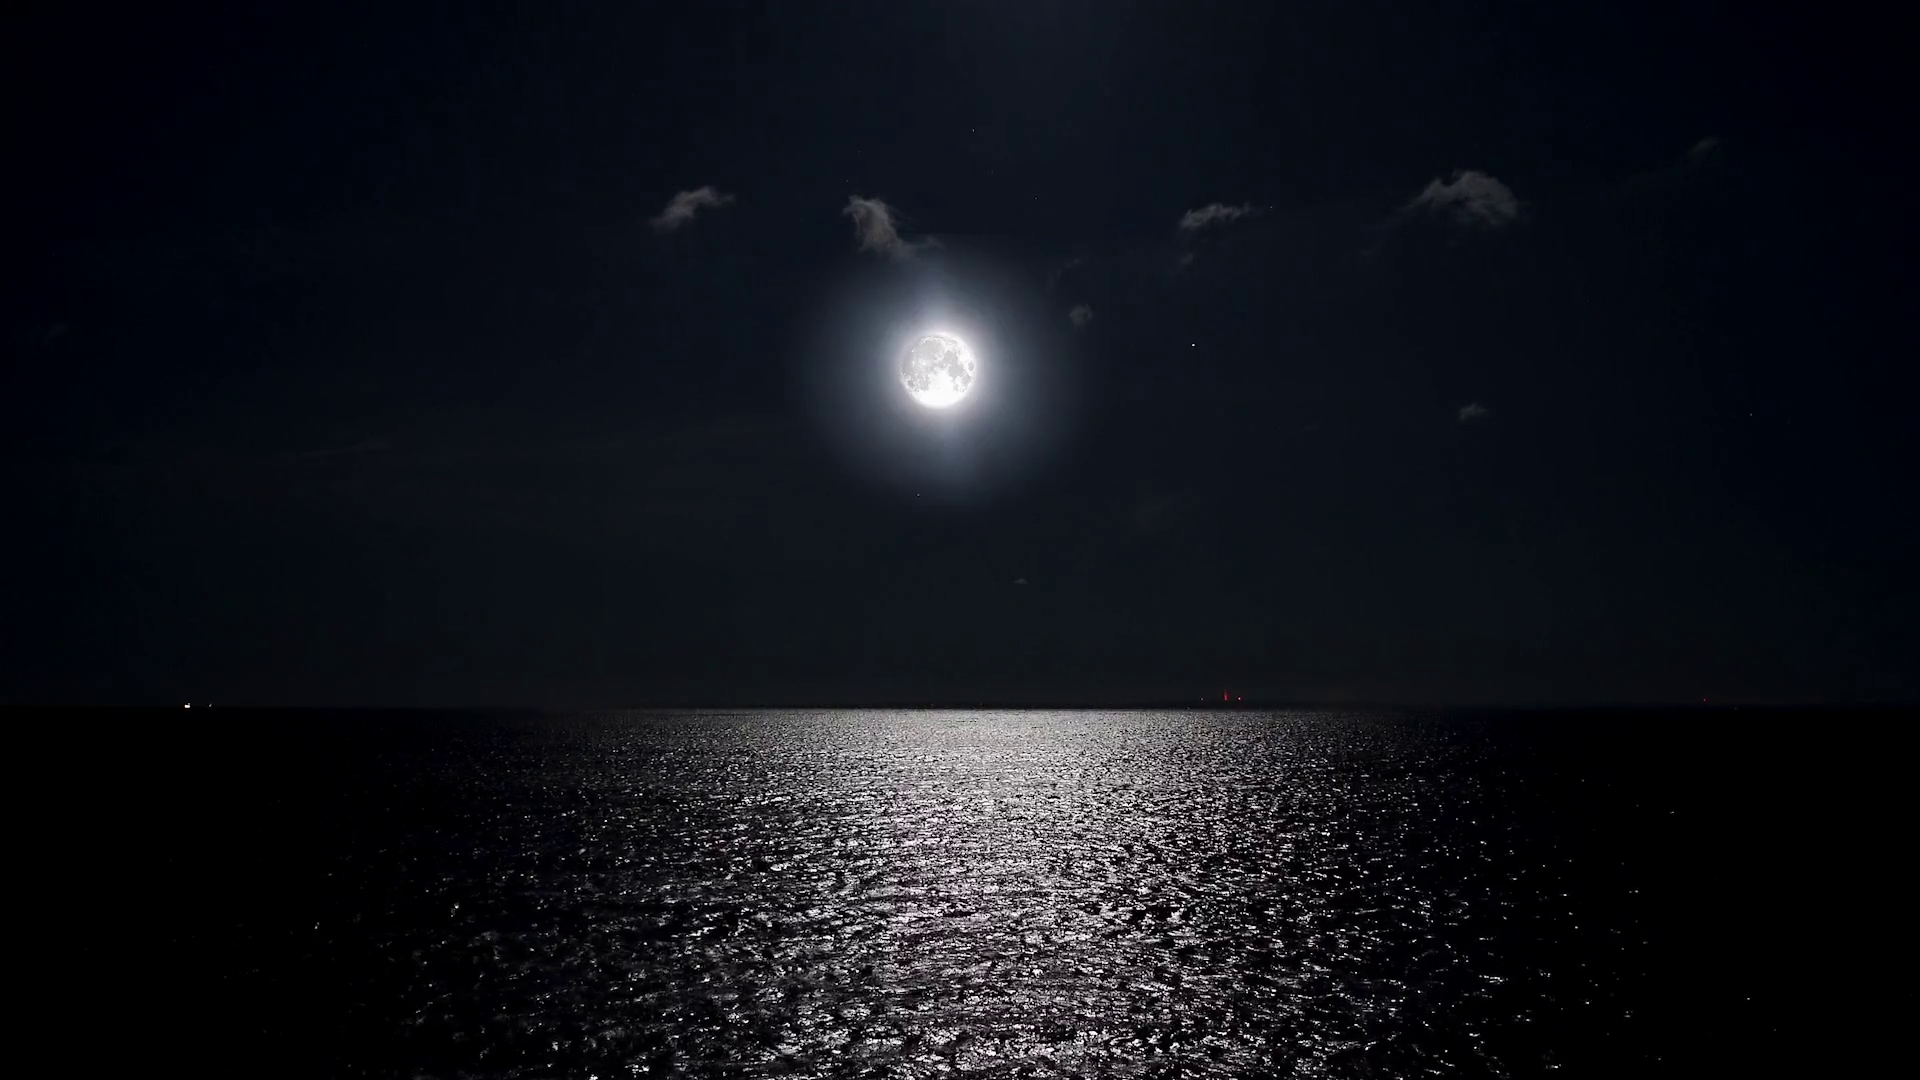
\includegraphics[scale=0.18]{10.png}
	\end{center}
\end{frame}

\begin{frame}
	\begin{center}
		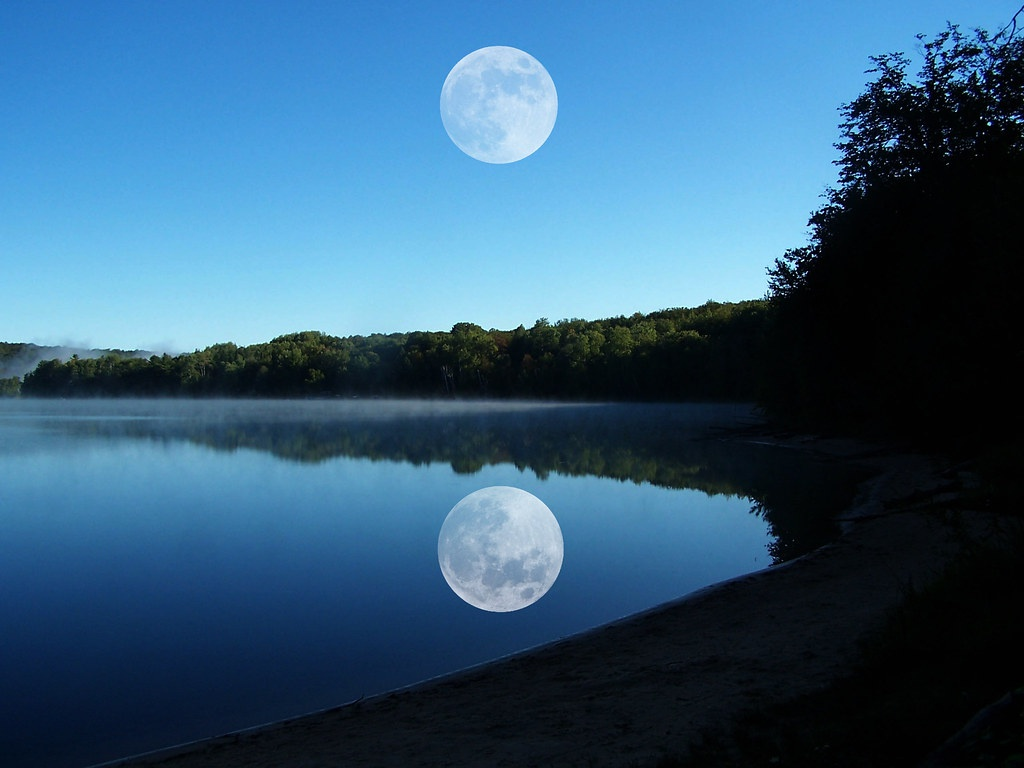
\includegraphics[scale=0.3]{11.jpeg}
	\end{center}
\end{frame}

\begin{frame}
	\begin{center}
		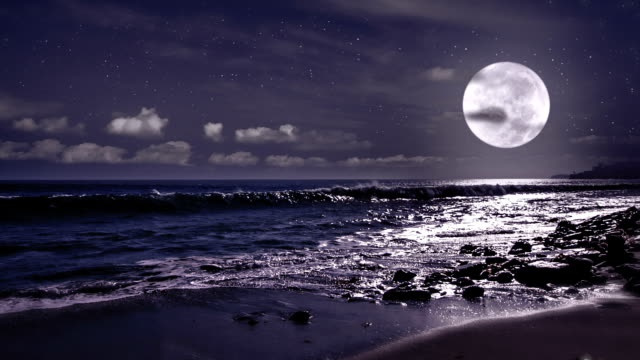
\includegraphics[scale=0.5]{12.jpeg}
	\end{center}
\end{frame}

\begin{frame}{Reflections: Mirror}
	\begin{center}
		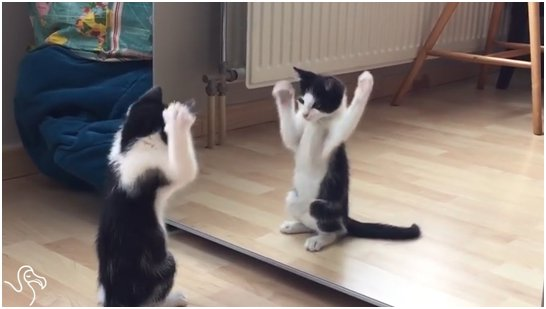
\includegraphics[scale=0.5]{14.jpeg}
	\end{center}
\end{frame}

\begin{frame}
	\begin{center}
		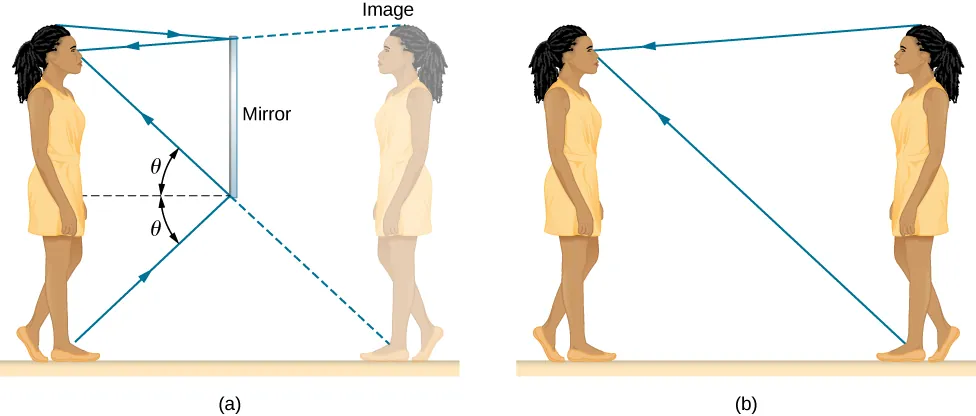
\includegraphics[scale=0.3]{13.png}
	\end{center}
\end{frame}

\begin{frame}{Reflections: Retroreflector}
	\begin{block}{Defenition}
		A \textbf{retroreflector} is a device or surface that reflects radiation (usually light) back to its source with minimum scattering
	\end{block} 
	What is the difference from a \textbf{planar mirror} ? \\

	This works in wide range of angle of incidence while mirror needs to be perpendicular to the wave front
	
\end{frame}

\begin{frame}{Retroreflector: Corner Cube Reflector}
% in documenet
\begin{center}
	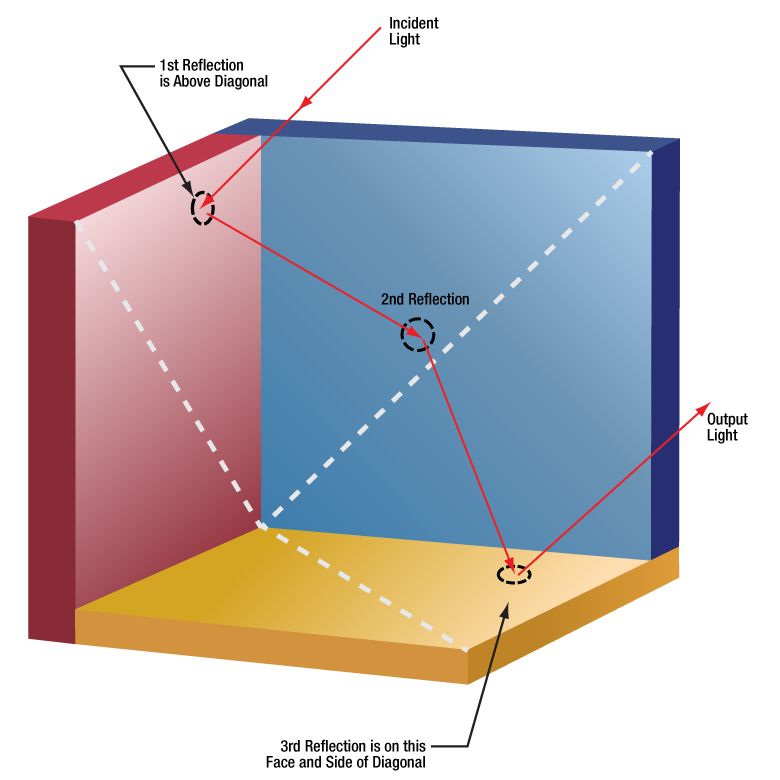
\includegraphics[scale=0.25]{15.png}
\end{center}
\end{frame}
\begin{frame}
\begin{center}
	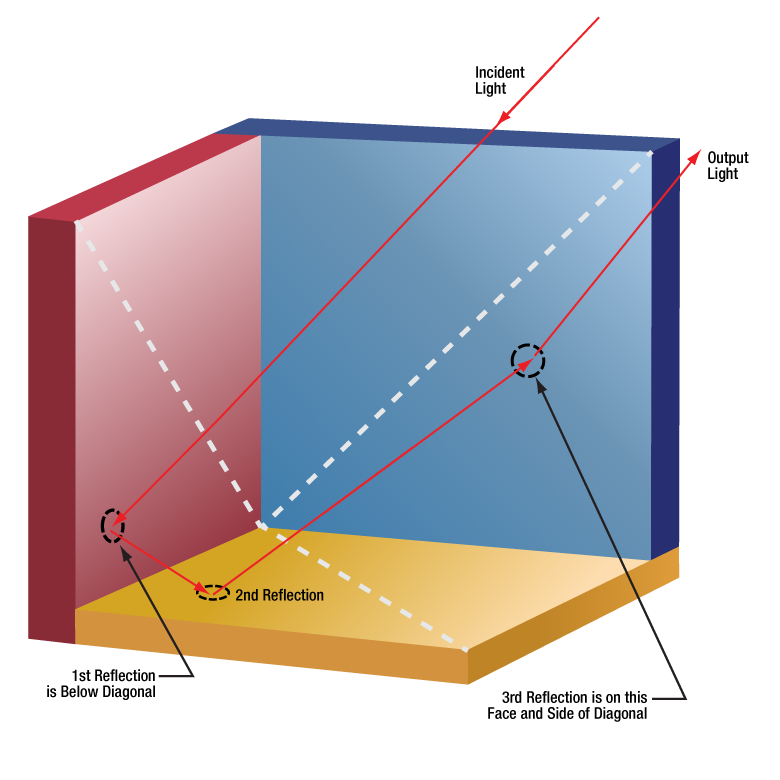
\includegraphics[scale=0.25]{20.png}
\end{center}
\end{frame}

\begin{frame}{Retroreflector : Uses}
	\begin{center}
		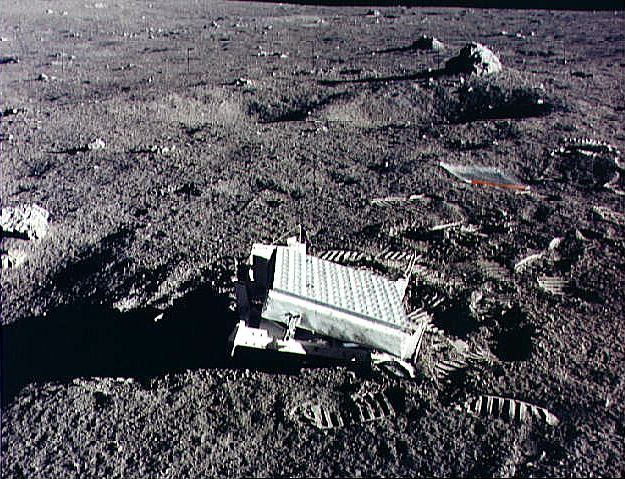
\includegraphics[scale=0.2]{21}
	\end{center}
	\begin{itemize}
		\item Astronauts placed a corner reflector on the Moon to measure its gradually increasing orbital distance. Laser signals from Earth can be bounced from that corner reflector to measure the gradually increasing distance to the Moon of a few centimeters per year.
	\end{itemize}
\end{frame}

\begin{frame}
	\begin{figure}
		\centering
		\begin{subfigure}[b]{0.4\textwidth}
			\centering
			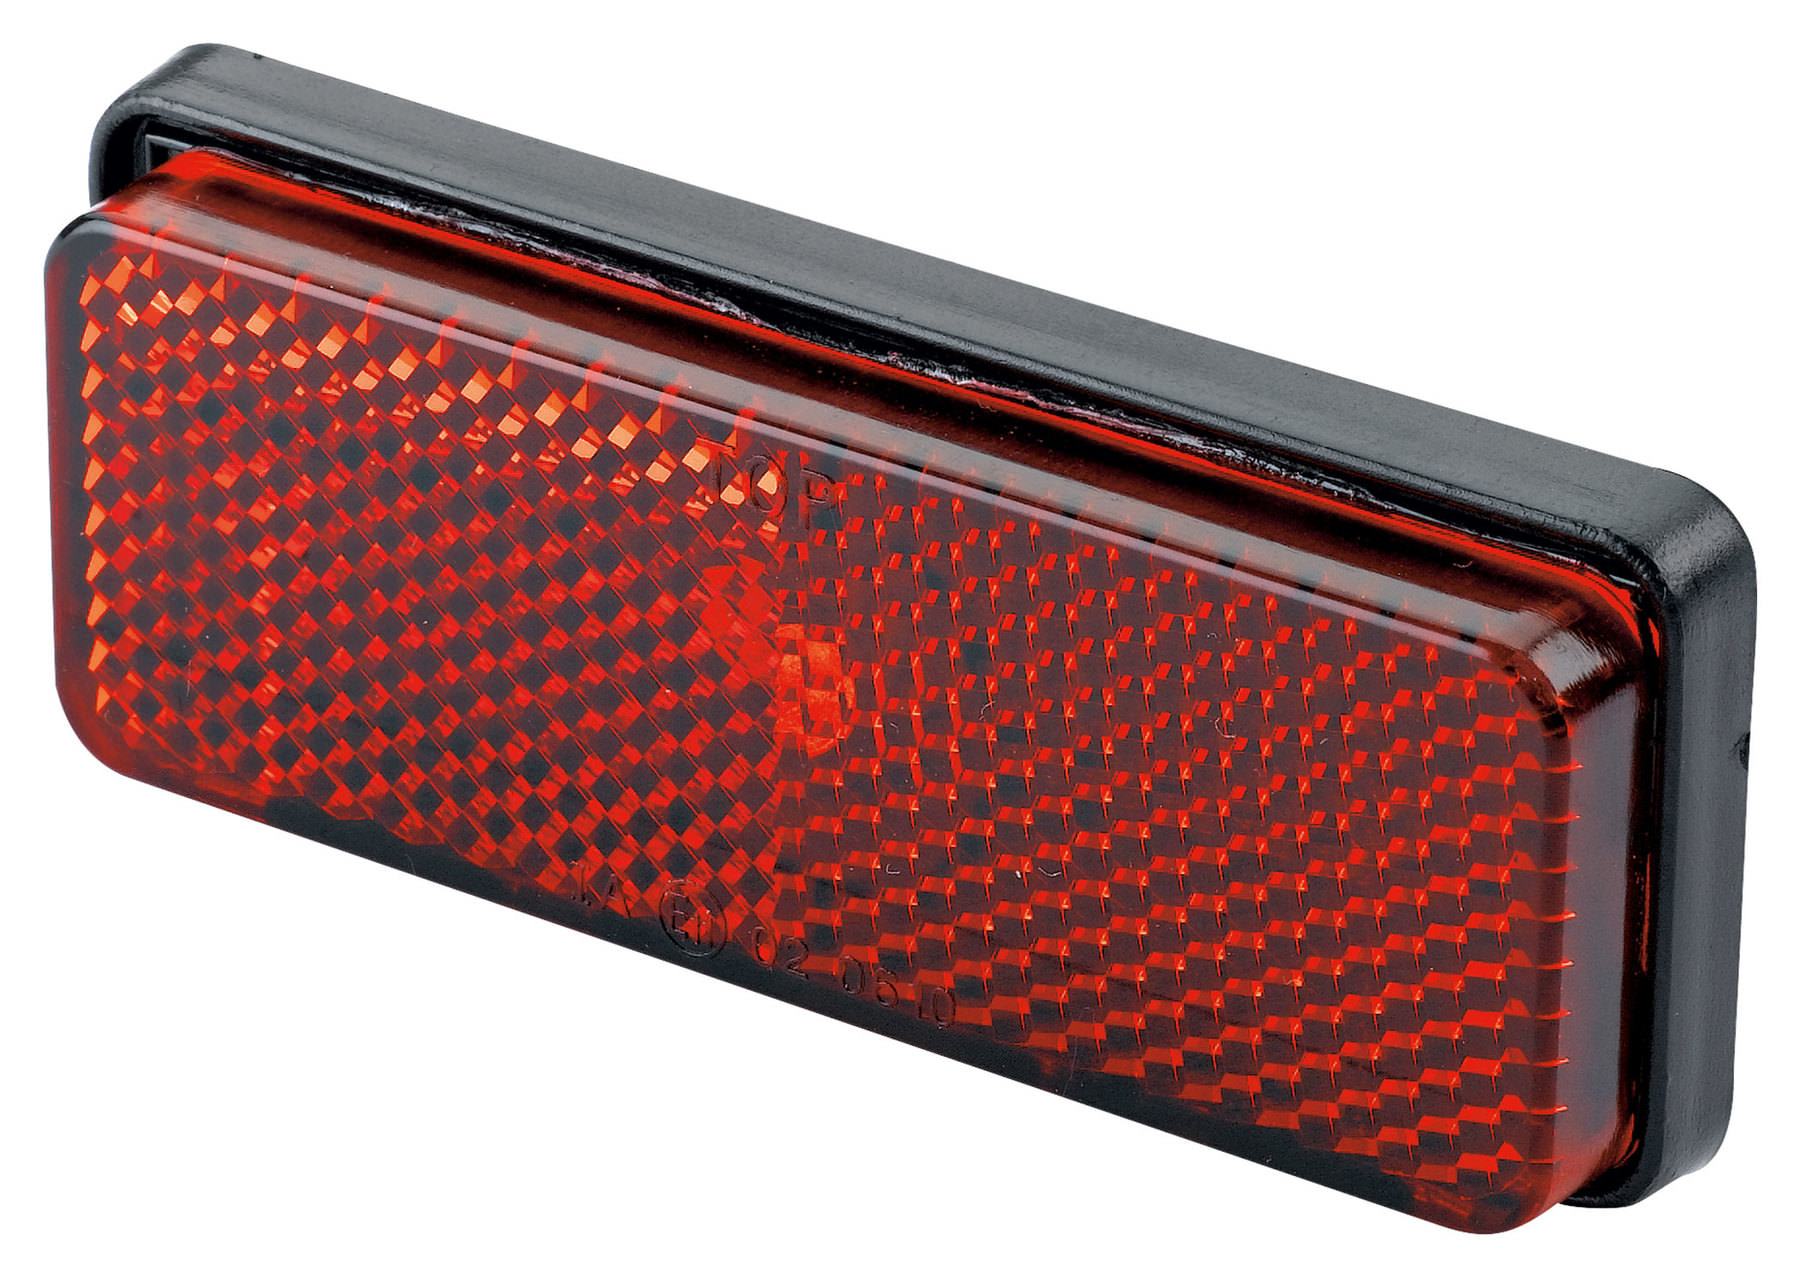
\includegraphics[width=\textwidth]{17.jpeg}
			\caption{cycle reflectors}
			\label{cycle reflectors}
		\end{subfigure}
		\hfill
		\begin{subfigure}[b]{0.4\textwidth}
			\centering
			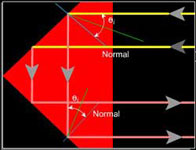
\includegraphics[width=\textwidth]{19.jpg}
			\caption{working principle}
			\label{fig:y equals x}
		\end{subfigure}
	\end{figure}
	\begin{itemize}
		\item Retroreflection ensures high visibility if the driver and the light source are located together in case of cycle reflectors
	\end{itemize}
\end{frame}
\begin{frame}{Retroreflector : Radar}
	\begin{center}
		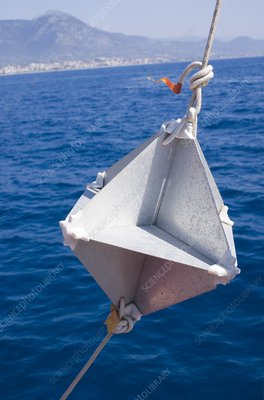
\includegraphics[scale=0.3]{22}
	\end{center}
	\begin{itemize}
		\item Small boats made of fiberglass or wood do not strongly reflect radio waves emitted by radar systems. To make these boats visible to radar (to avoid collisions, for example), radar reflectors are attached to boats, usually in high places
	\end{itemize}
\end{frame}
\subsection{Refraction}
	\begin{frame}{The actual location of Mug ?}
		\begin{center}
			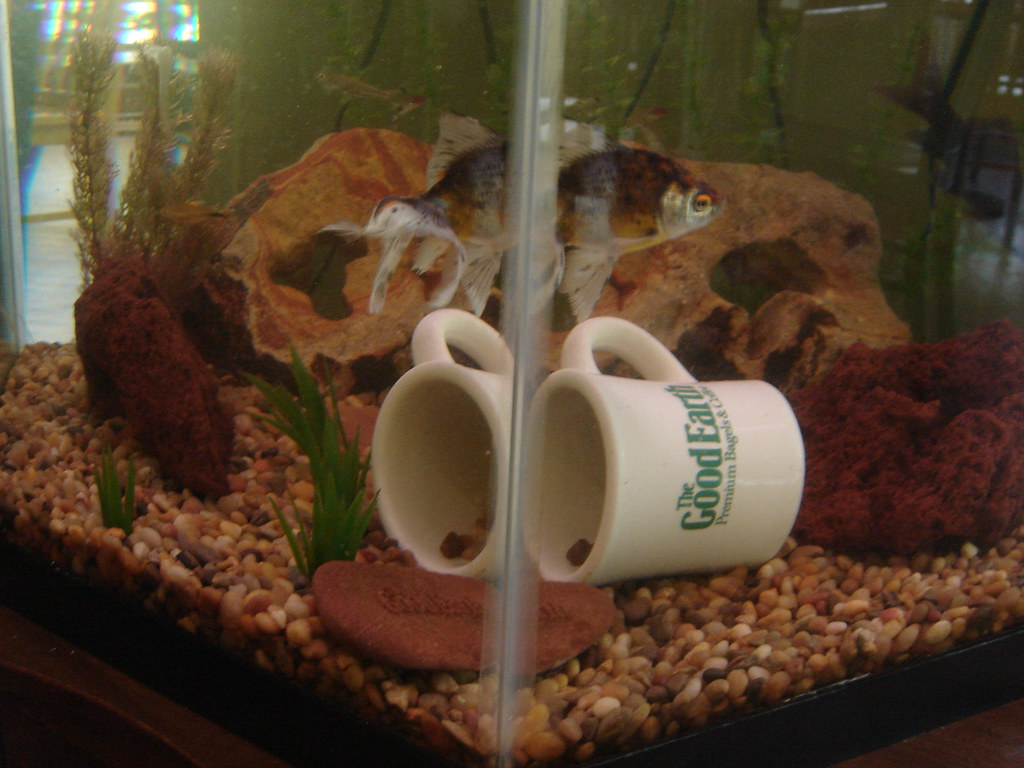
\includegraphics[scale=0.2]{23.jpeg}
		\end{center}
		\pause
		\begin{center}
			Both are not the actual location !!!
		\end{center}
	\end{frame}
	\begin{frame}{Why two mugs ?}
		\begin{block}{Refraction}
			The changing of a light ray’s direction (loosely called bending) when it passes through substances of different refractive indices is called \textbf{refraction}
		\end{block}
		\pause
		\begin{center}
			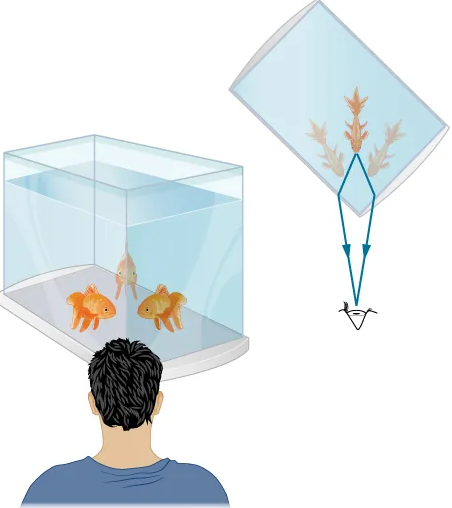
\includegraphics[scale=0.28]{24.png}
		\end{center}
	\end{frame}
\begin{frame}
	\begin{block}{Velocity of Light}
		\begin{displaymath}
			v = c/\eta
		\end{displaymath}
	\end{block}
	\begin{figure}
		\centering
		\begin{subfigure}[b]{0.42\textwidth}
			\centering
			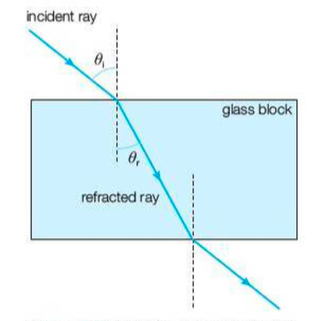
\includegraphics[width=\textwidth]{25.png}
			\caption{Refraction through a glass block}
			\label{Refraction}
		\end{subfigure}
		\hfill
		\begin{subfigure}[b]{0.5\textwidth}
			\centering
			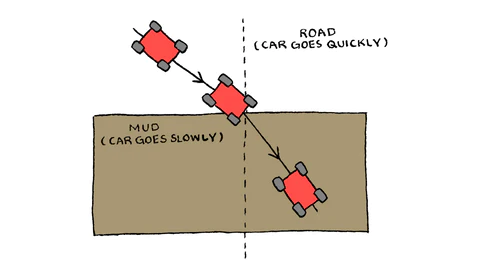
\includegraphics[width=\textwidth]{26.png}
			\caption{Direction of Bending}
			\label{Bending Direction}
		\end{subfigure}
	\end{figure}
\end{frame}

\begin{frame}
\begin{block}{Snell's Law}
	\begin{displaymath}
		\eta_{1} \sin\theta_{1} = \eta_{2} \sin\theta_{2}
	\end{displaymath}
\end{block}
\end{frame}
\subsection{Total Internal Reflection}
\begin{frame}
	\begin{center}
		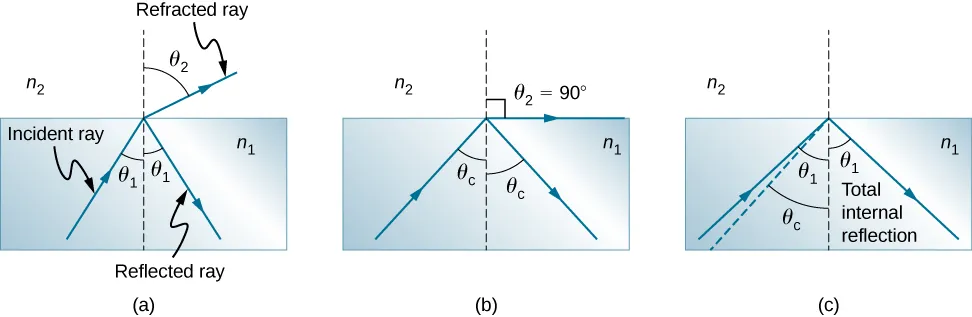
\includegraphics[scale=0.3]{28.png}
	\end{center}
	\begin{enumerate}
		\item[a.] $\eta_{1} > \eta_{2} \implies \theta_{2} < \theta_{1}$
		\item[b.]  $\theta_{1} \uparrow \implies \theta_{2} \uparrow $. At $\theta_{1} = \theta_{c}, \theta_{2} = 90\degree$
		\item[c.] At $\theta_{1} > \theta_{c}$, all of the light is reflected back in to medium $=$ \textbf{total internal reflection}  
	\end{enumerate}
	\begin{displaymath}
		\theta_{c} = \sin^{-1}\left( \frac{\eta_{1}}{\eta_{2}} \right) \text{for}\; \eta_{1} > \eta_{2}
	\end{displaymath}
\end{frame}
\begin{frame}{What is happening here?}
	\begin{center}
		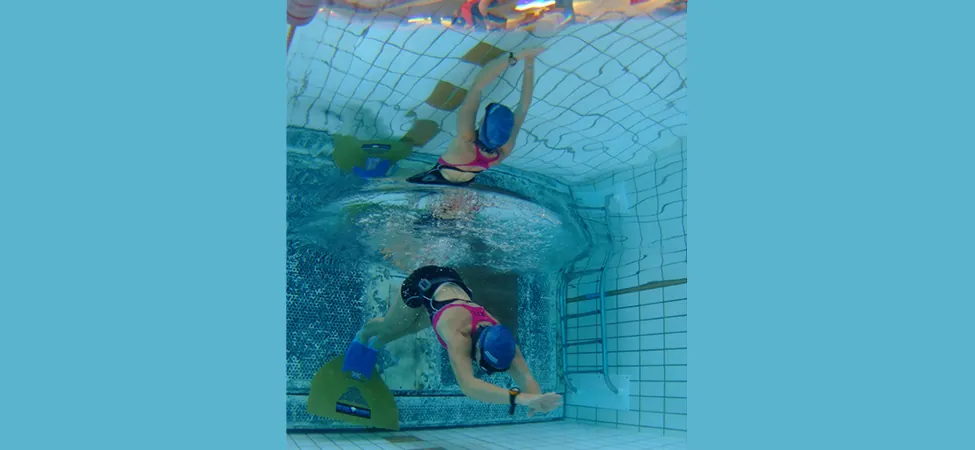
\includegraphics[scale=0.3]{30.png}
	\end{center}
\end{frame}


\begin{frame}{Fiber Optical Cables and Endoscopes}
	\begin{figure}
		\centering
		\begin{subfigure}[b]{0.3\textwidth}
			\centering
			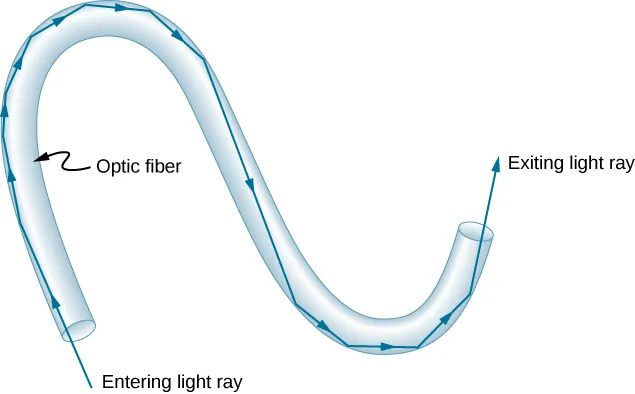
\includegraphics[width=\textwidth]{31.png}
			\caption{Total internal reflection in fiber optic cable}
			\label{Refraction}
		\end{subfigure}
		\hfill
		\begin{subfigure}[b]{0.3\textwidth}
			\centering
			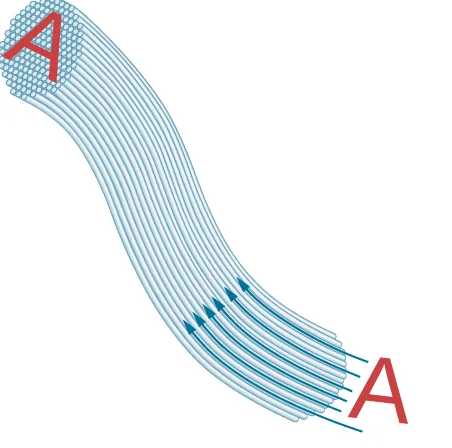
\includegraphics[width=\textwidth]{32.png}
			\caption{Bundle of Fiber optic cables}
			\label{Bending Direction}
		\end{subfigure}
			\hfill
			\begin{subfigure}[b]{0.3\textwidth}
				\centering
				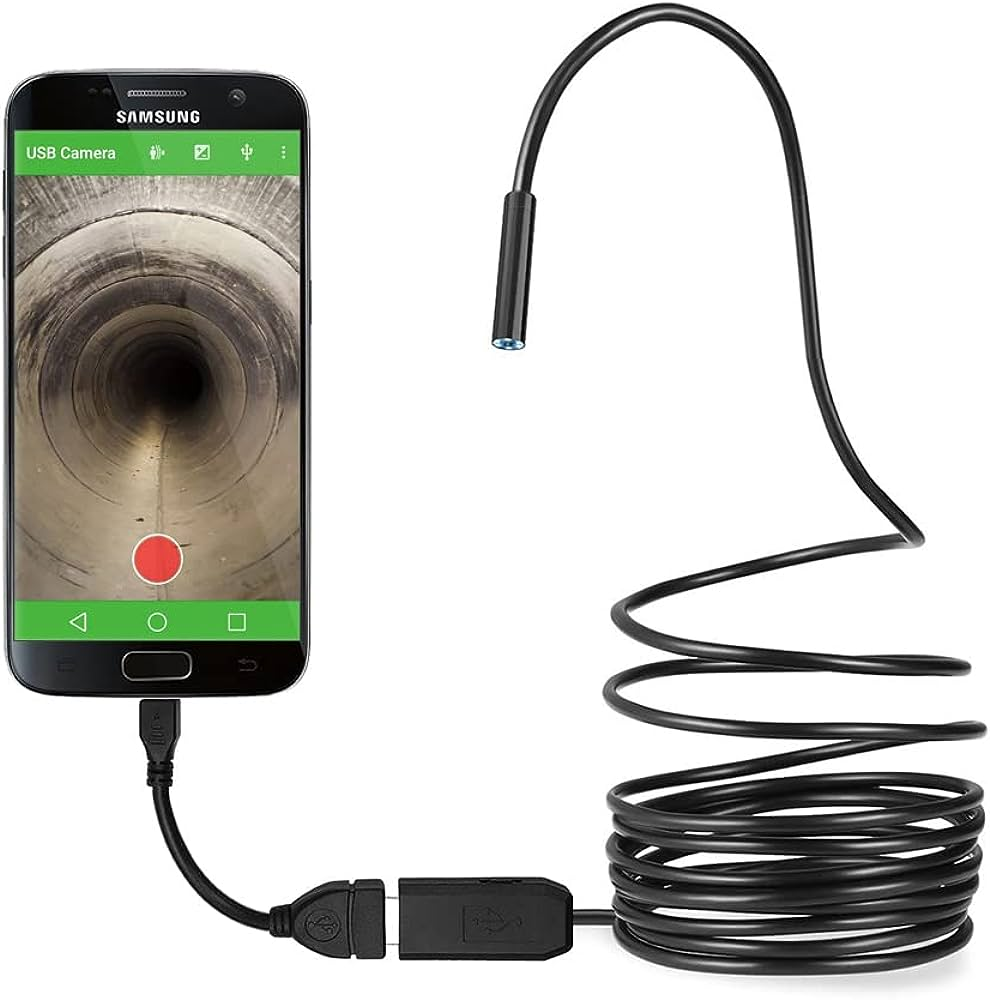
\includegraphics[width=\textwidth]{33.jpg}
				
				\caption{Endoscospic Camera}
				\label{Bending Direction}
			\end{subfigure}
	\end{figure}

\end{frame}

\section{Huygen's Principle}

\begin{frame}
	\frametitle{Premise}
	\begin{itemize}
		\item Light behaves as both wave and particle 
		\item Some optical phenomena require analysis based on wave characteristics of light when the wavelength is not negligible compared to dimension of optical device e.g. slit in case of \alert{diffraction} 
	\end{itemize}
\end{frame}

\section{Polarization}
\begin{frame}
	\begin{center}
		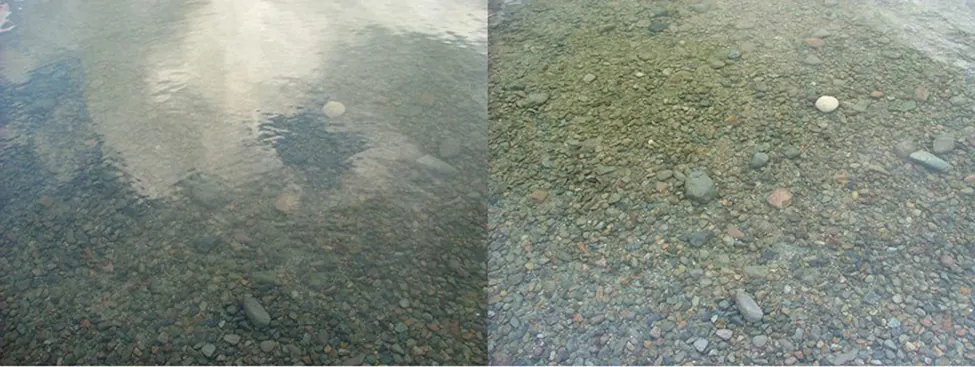
\includegraphics[scale=0.3]{33.png}
	\end{center}
	\begin{enumerate}
		\item [a.] glare effect 
		\item [b.] using polarizing filter . this reduces the glare
	\end{enumerate}
\end{frame}
\begin{frame}
	\begin{center}
		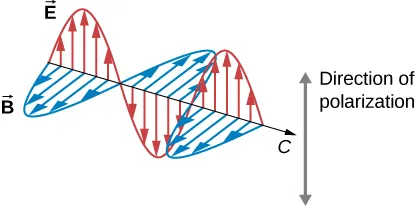
\includegraphics[scale=0.8]{34.png}
	\end{center}
\end{frame}
\begin{frame}
	\frametitle{EM wave propagation}
	\begin{itemize}
		\item EM waves are transverse waves consisting of varying Electric and Magnetic fields that oscillate perpendicular to the direction of propagation
	
		\item \alert{Polarization} is the attribute that a wave’s oscillations do have a definite direction relative to the direction of propagation of the wave
		
		\item For an EM wave, the direction of polarization is the direction parallel to the electric field.
	\end{itemize}
\end{frame}
\begin{frame}{Vertical vs Horizontal Polarization}
	\begin{center}
		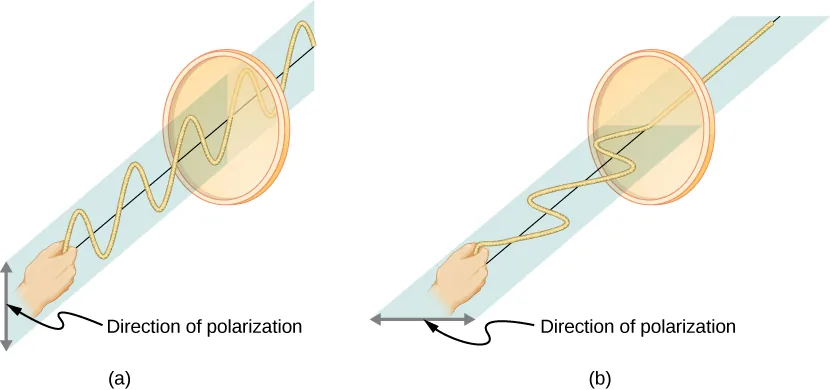
\includegraphics[scale=0.3]{35.png}
	\end{center}
	\begin{enumerate}
		\item[a.] Vertical polarization . Effect of vertical slit placed on the rope and the waves will pass through
		\item[b.] Horizontal polarization. Effect of horizontal slit where the wave propagation got blocked 
	\end{enumerate}
\end{frame}

\begin{frame}
	\frametitle{Polarizing filter}
	\begin{center}
		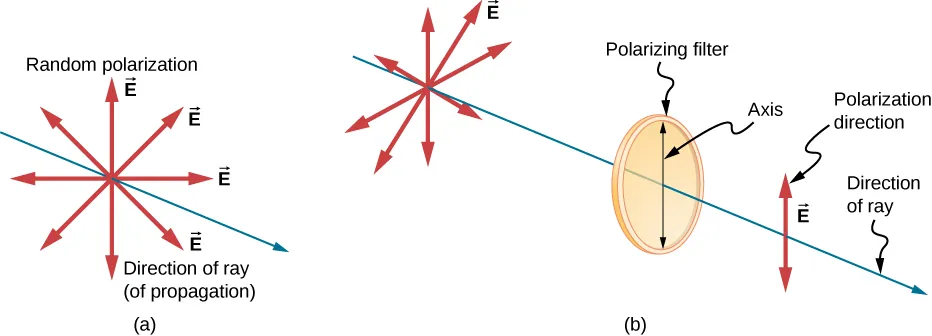
\includegraphics[scale=0.3]{36.png}
	\end{center}
\end{frame}

\section{Geometric Optics}
\subsection{Image formation in Plane Mirrors}
\begin{frame}
	\begin{center}
		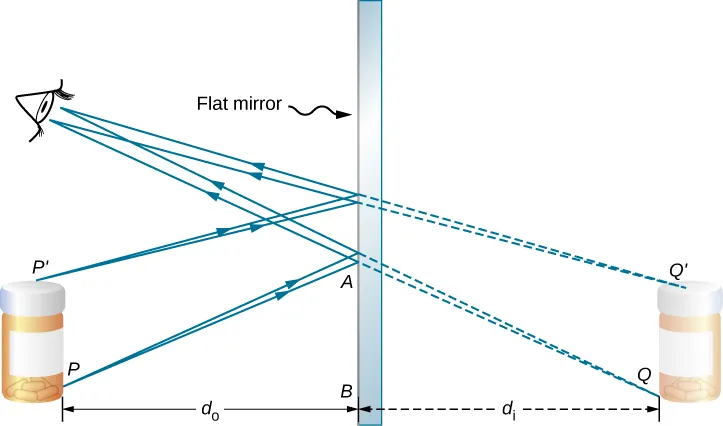
\includegraphics[scale=0.3]{37.png}
	\end{center}
	\begin{displaymath}
		d_{o} = -d_{i} 
	\end{displaymath}
\end{frame}
\begin{frame}{Multiple Images: infinite }
	\begin{center}
		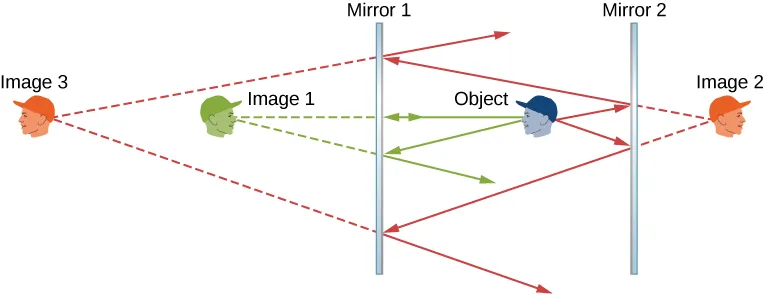
\includegraphics[scale=0.4]{38.png}
	\end{center}
\end{frame}
\begin{frame}{Multiple Images: finite }
	\begin{center}
		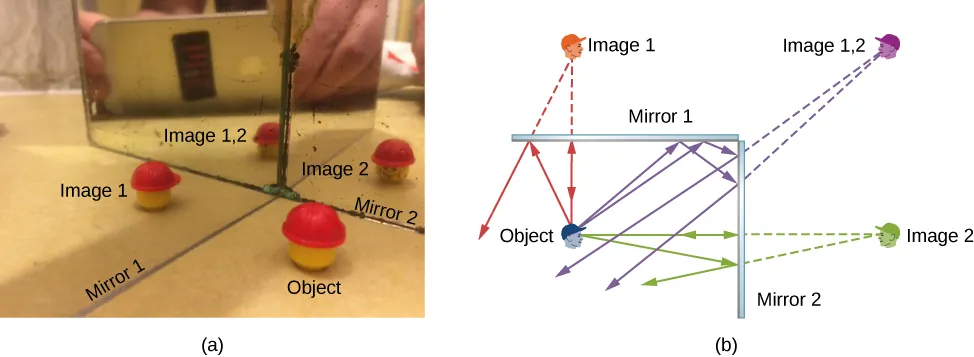
\includegraphics[scale=0.3]{39.png}
	\end{center}
\end{frame}
\subsection{Spherical Mirrors}
\begin{frame}{Curved Mirrors }
	\begin{itemize}
		\item A \textbf{curved mirror} can form images that may be larger or smaller than the object and may form either in front of the mirror or behind it.
	\end{itemize}
	
\end{frame}
\end{document}
